\clearpage
\section{Class Diagram}\label{sec:class-diagram}

Il diagramma dei package della sezione~\ref{sec:package-diagram} è dettagliato in quattro diagrammi di classe. Le figure mantengono i colori dei livelli e riportano i membri essenziali alla lettura delle dipendenze.

\subsection{Domain Model}

Il dominio comprende catalogo, utenti, operazioni ed eventi di inventario. \code{Vehicle} controlla alcune transizioni di stato e \code{BankAccount} verifica il saldo nei prelievi. \code{User}, \code{Vehicle}, \code{Request}, \code{Sale}, \code{Rent} e \code{TestDrive} derivano da \code{BaseEntity}; nel disegno compaiono solo tre generalizzazioni per evitare sovrapposizioni. I riferimenti fra entità usano ID, non associazioni Java dirette. \code{Vehicle.transitionTo} consente anche cambi di stato generici.

\begin{figure}[H]
  \centering
  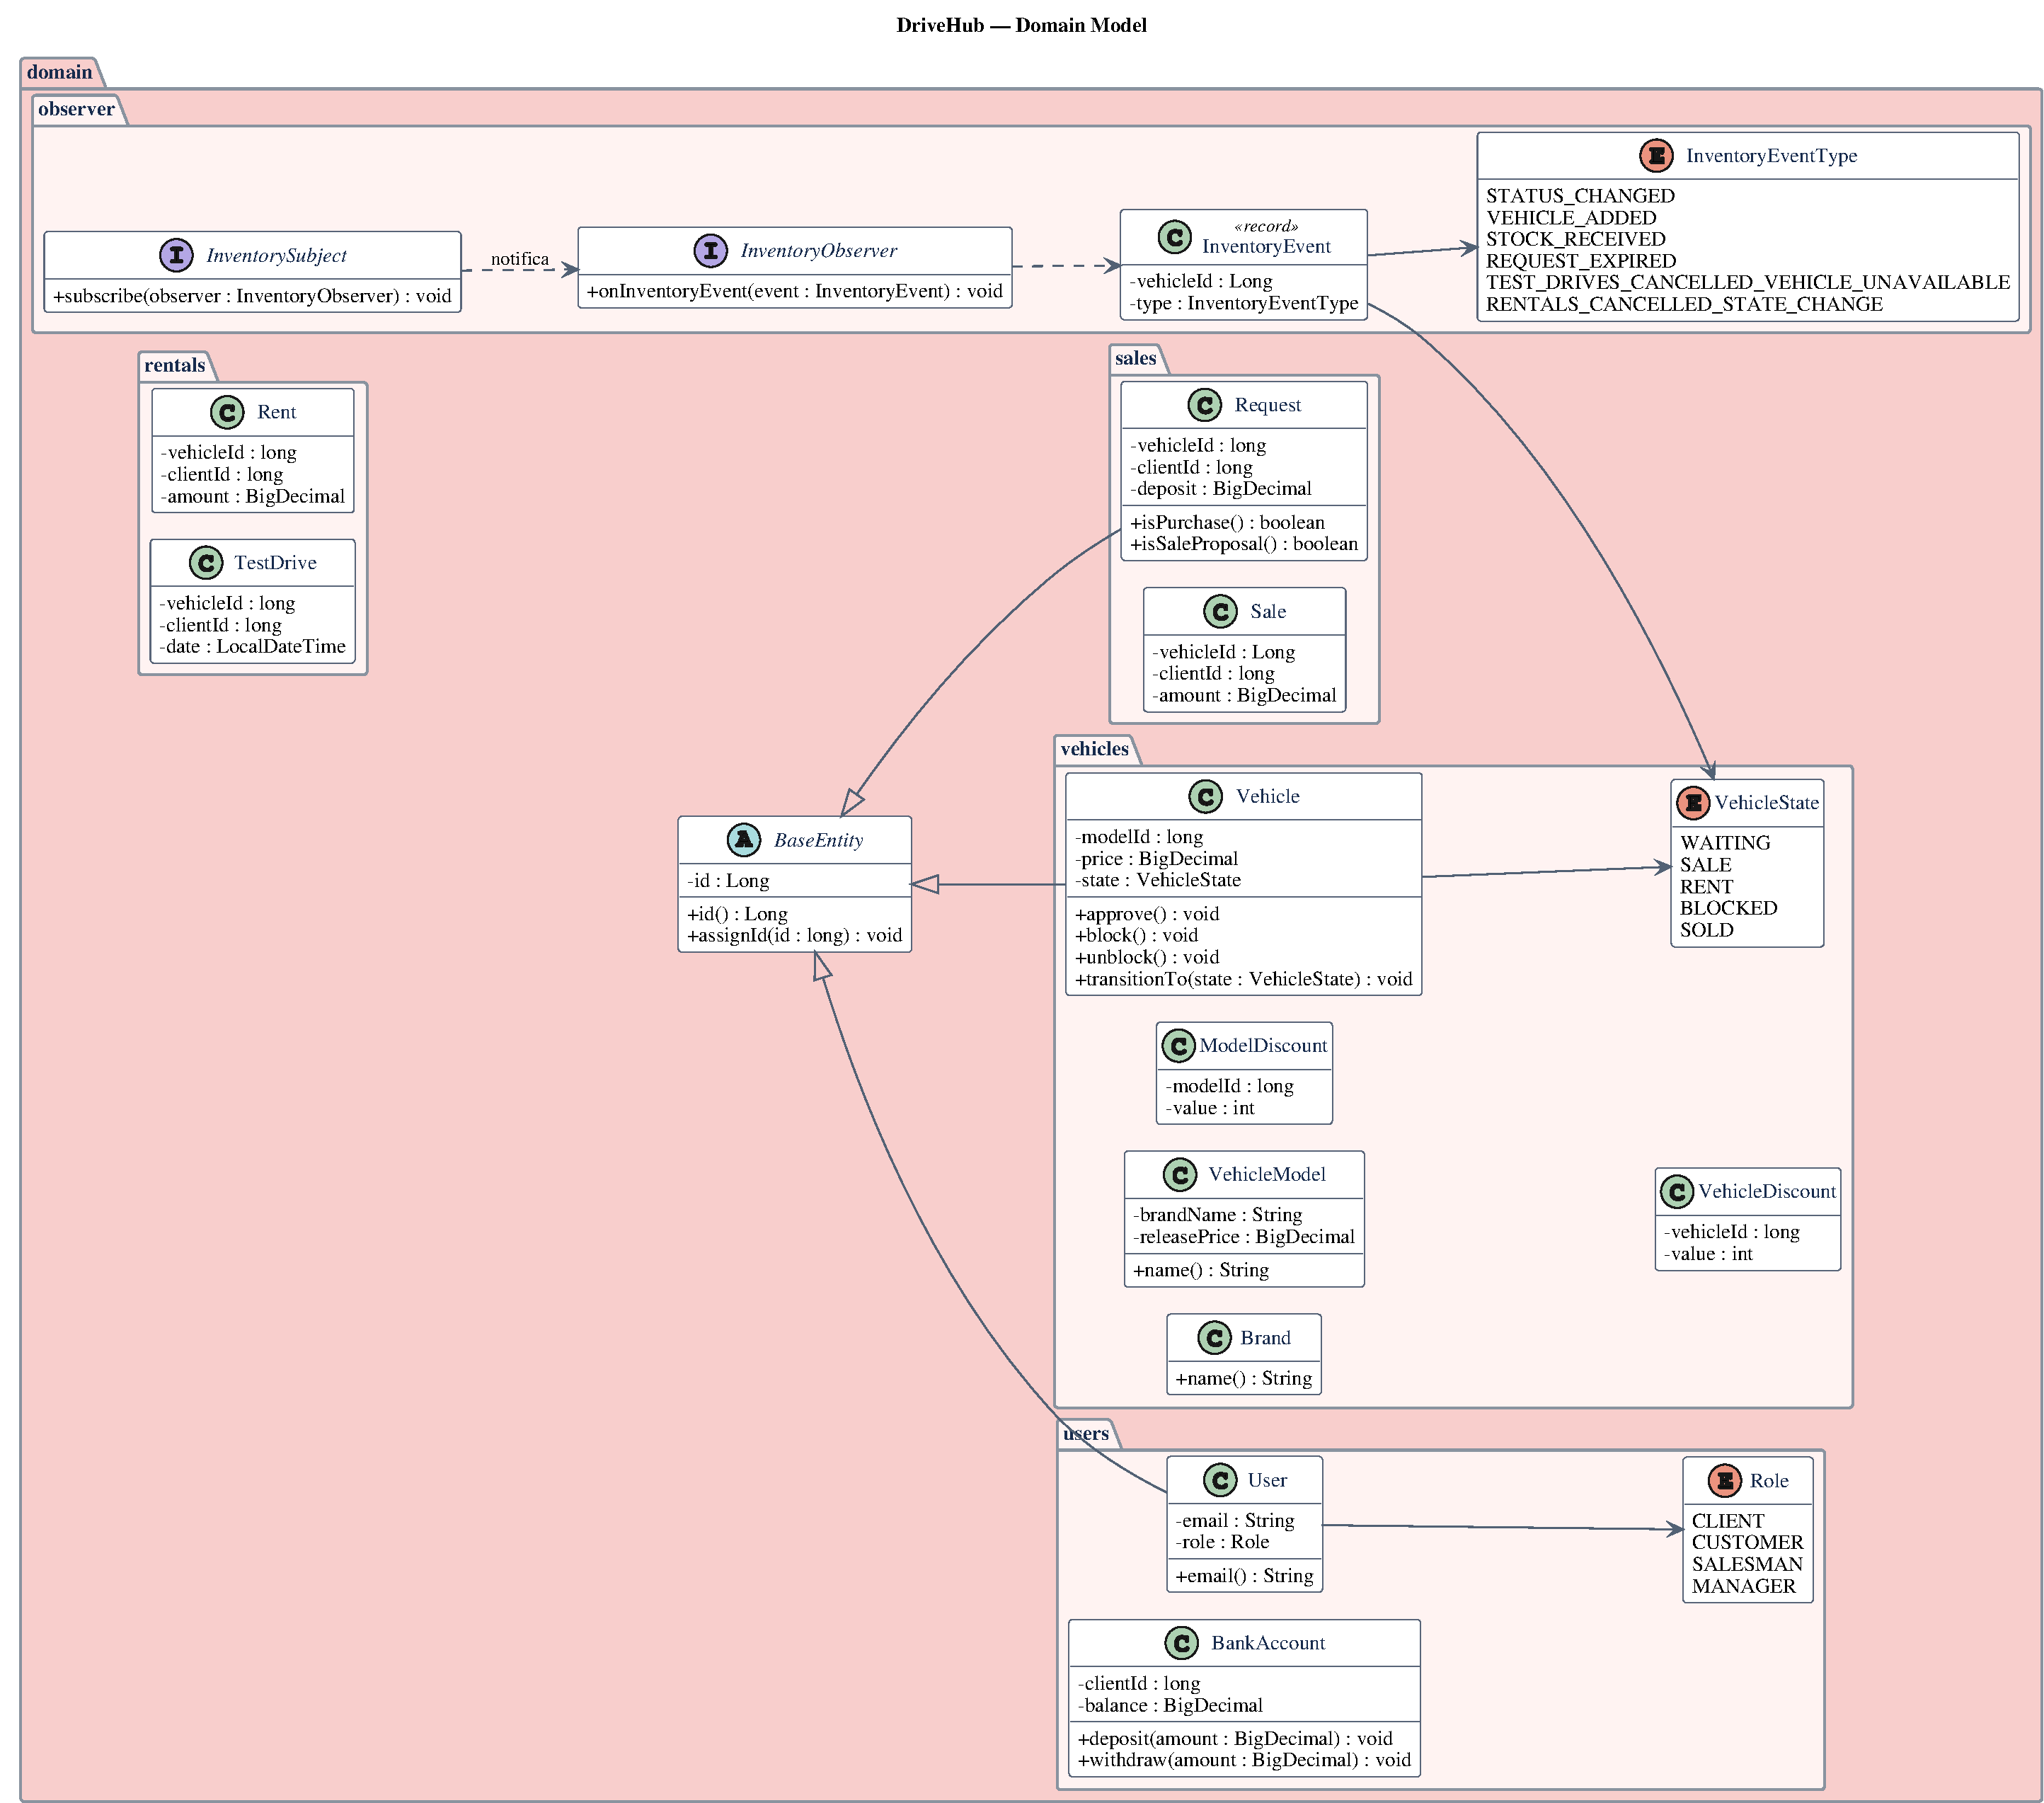
\includegraphics[width=\textwidth,height=.59\textheight,keepaspectratio]{class-domain-drivehub.pdf}
  \caption{Domain Model di DriveHub: classi rappresentative dei package interni al dominio.}\label{fig:classi-domain}
\end{figure}

\clearpage
\subsection{Business Layer}

I servizi coordinano i casi d'uso dell'applicazione. \code{TransactionRunner} apre una \code{UnitOfWork} tramite \code{DaoFactory}, così le operazioni correlate possono condividere una transazione. \code{PricingService} delega i calcoli a \code{PricingStrategy}, implementata da \code{StandardPricingStrategy}; \code{AuthService} usa \code{PasswordHasher} per le credenziali. \code{SalesService} e \code{RentalService} implementano \code{InventorySubject} e notificano gli \code{InventoryObserver}. Nel diagramma le piccole aree blu e rosse mostrano le interfacce degli altri livelli usate dal business.

\begin{figure}[H]
  \centering
  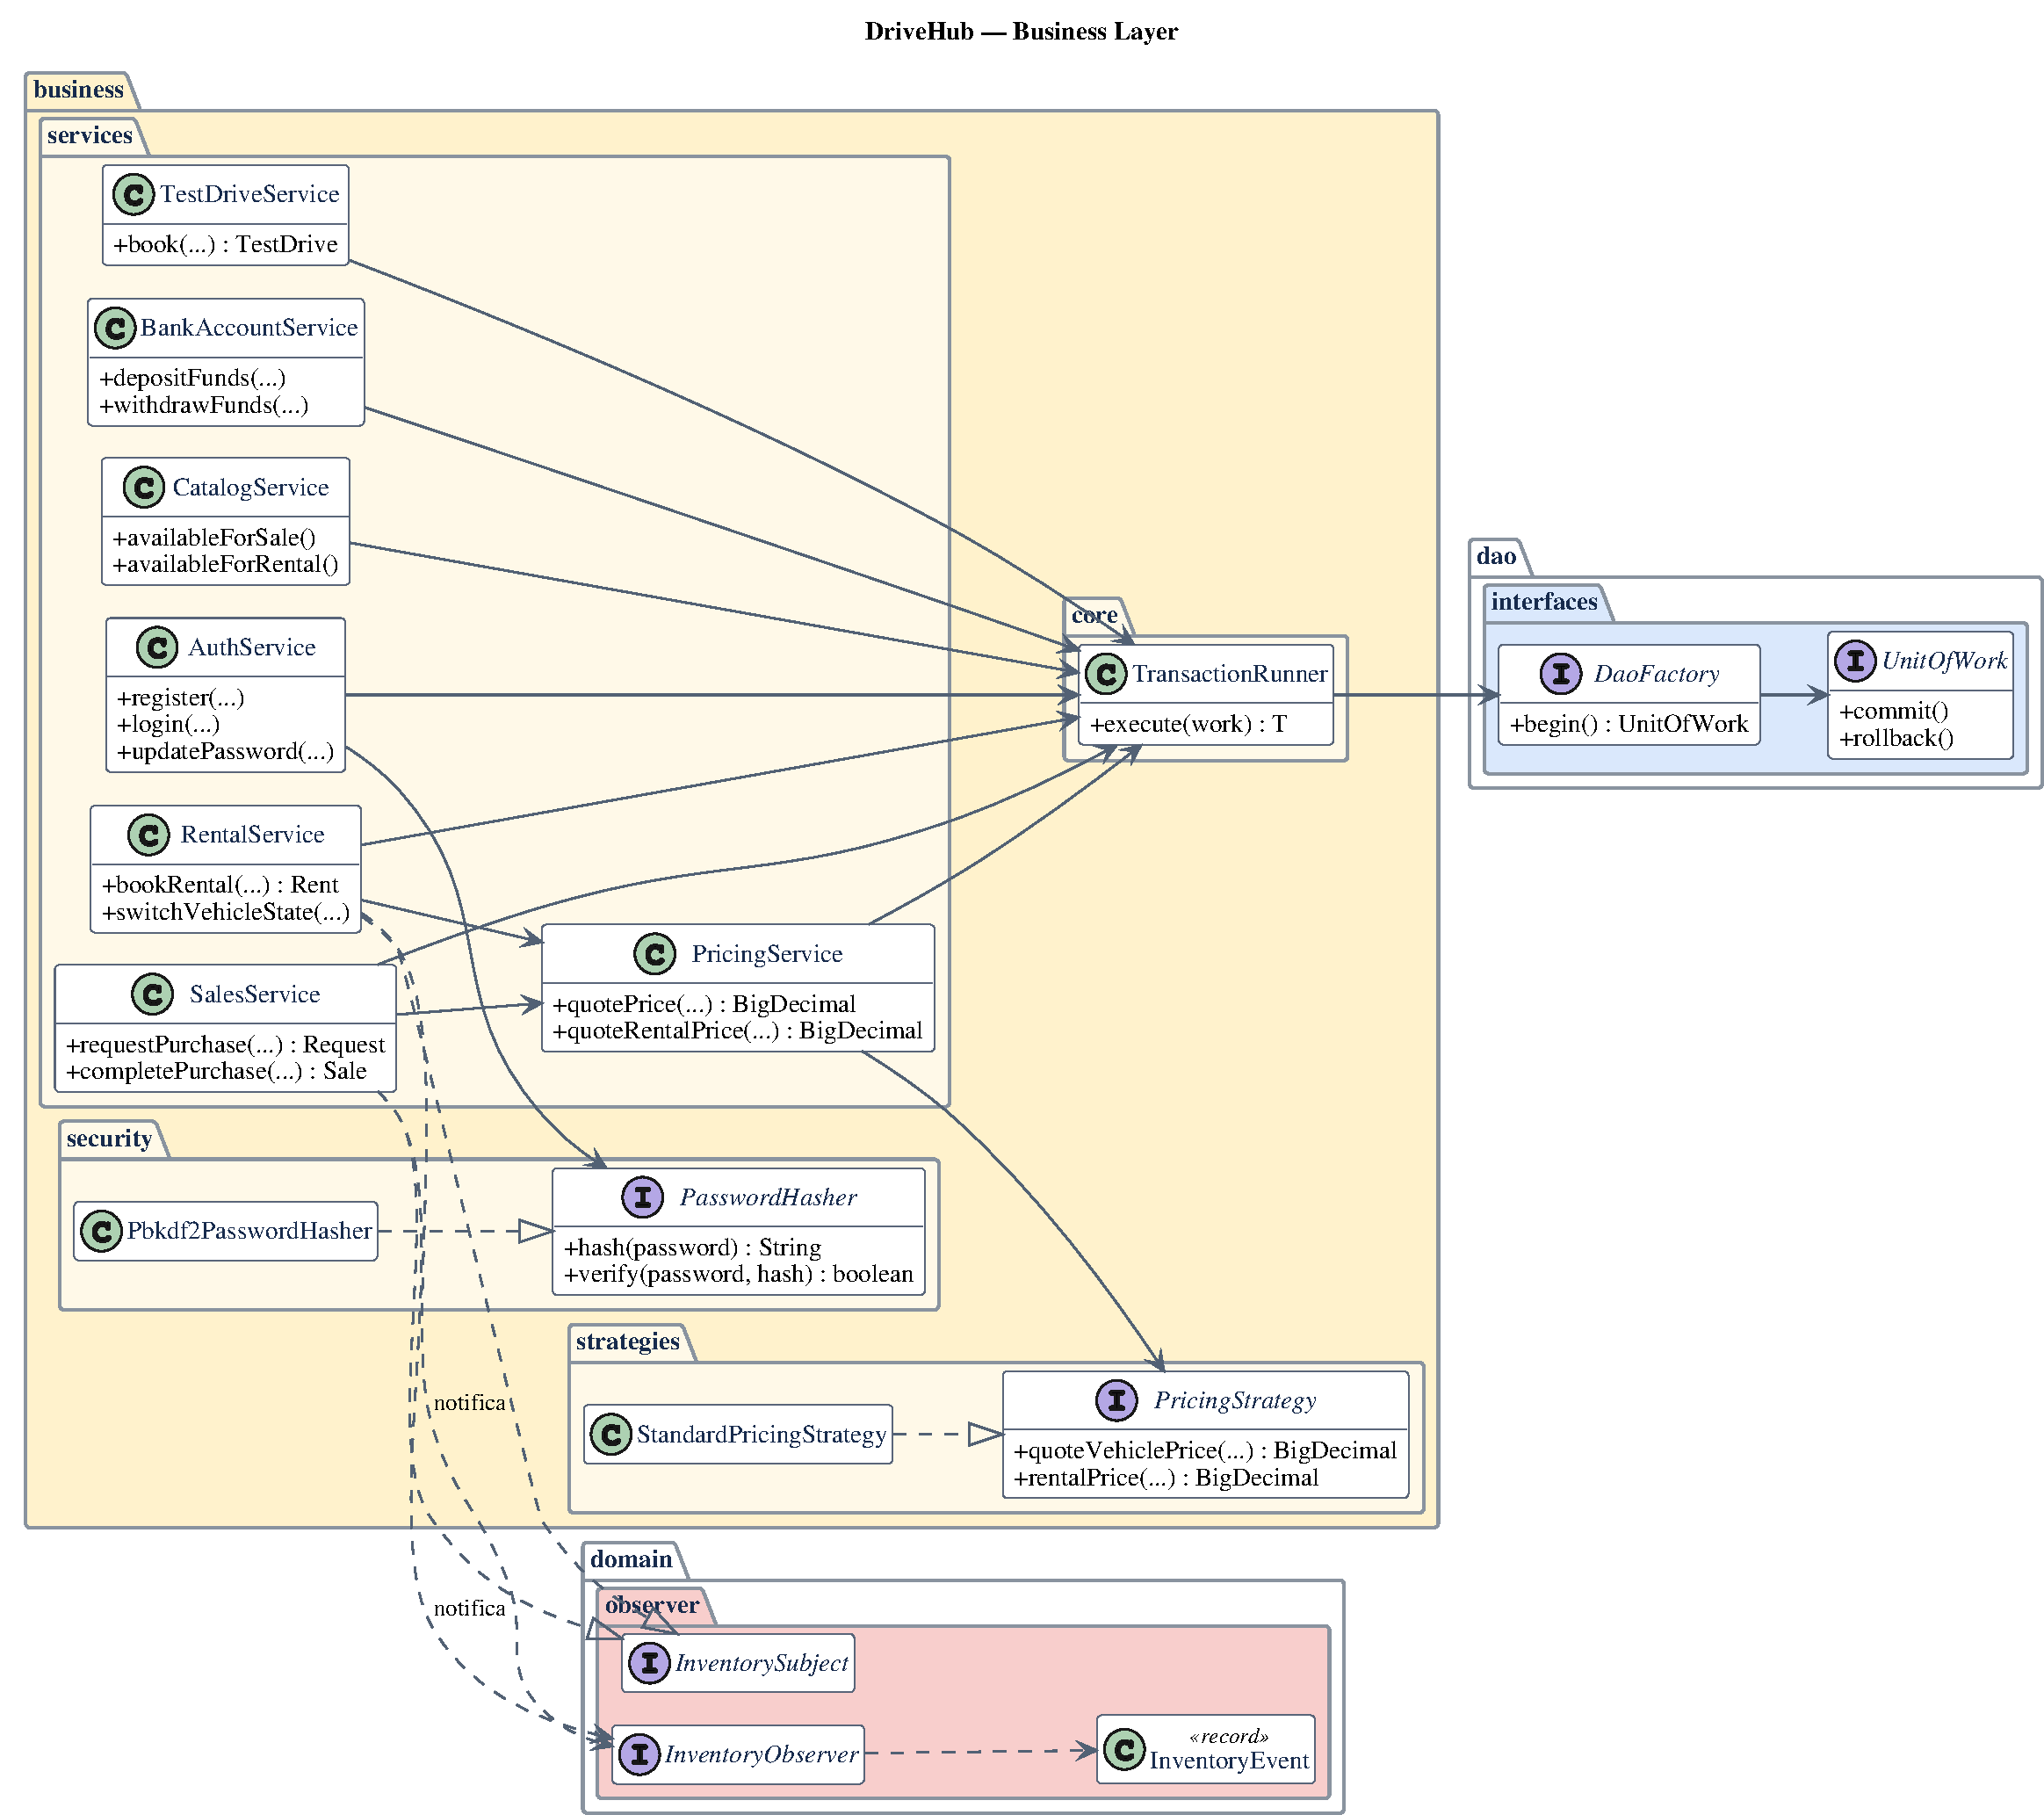
\includegraphics[width=\textwidth,height=.72\textheight,keepaspectratio]{class-business-drivehub.pdf}
  \caption{Business Layer: servizi, transazioni, Strategy e Observer.}\label{fig:classi-business}
\end{figure}

\clearpage
\subsection{DAO}

Il DAO separa le porte di persistenza dalle classi che eseguono le query JDBC. \code{PostgresDaoFactory.begin} crea una \code{PostgresUnitOfWork}; questa espone i DAO che condividono la connessione e offre \code{commit} e \code{rollback}. Il diagramma mostra quattro coppie interfaccia--implementazione come esempio. Le altre sei porte, per conti, marchi, modelli, sconti, test drive e vendite, seguono lo stesso schema. \code{JdbcEntityLoader} collabora alla ricostruzione degli oggetti dai risultati SQL.

\begin{figure}[H]
  \centering
  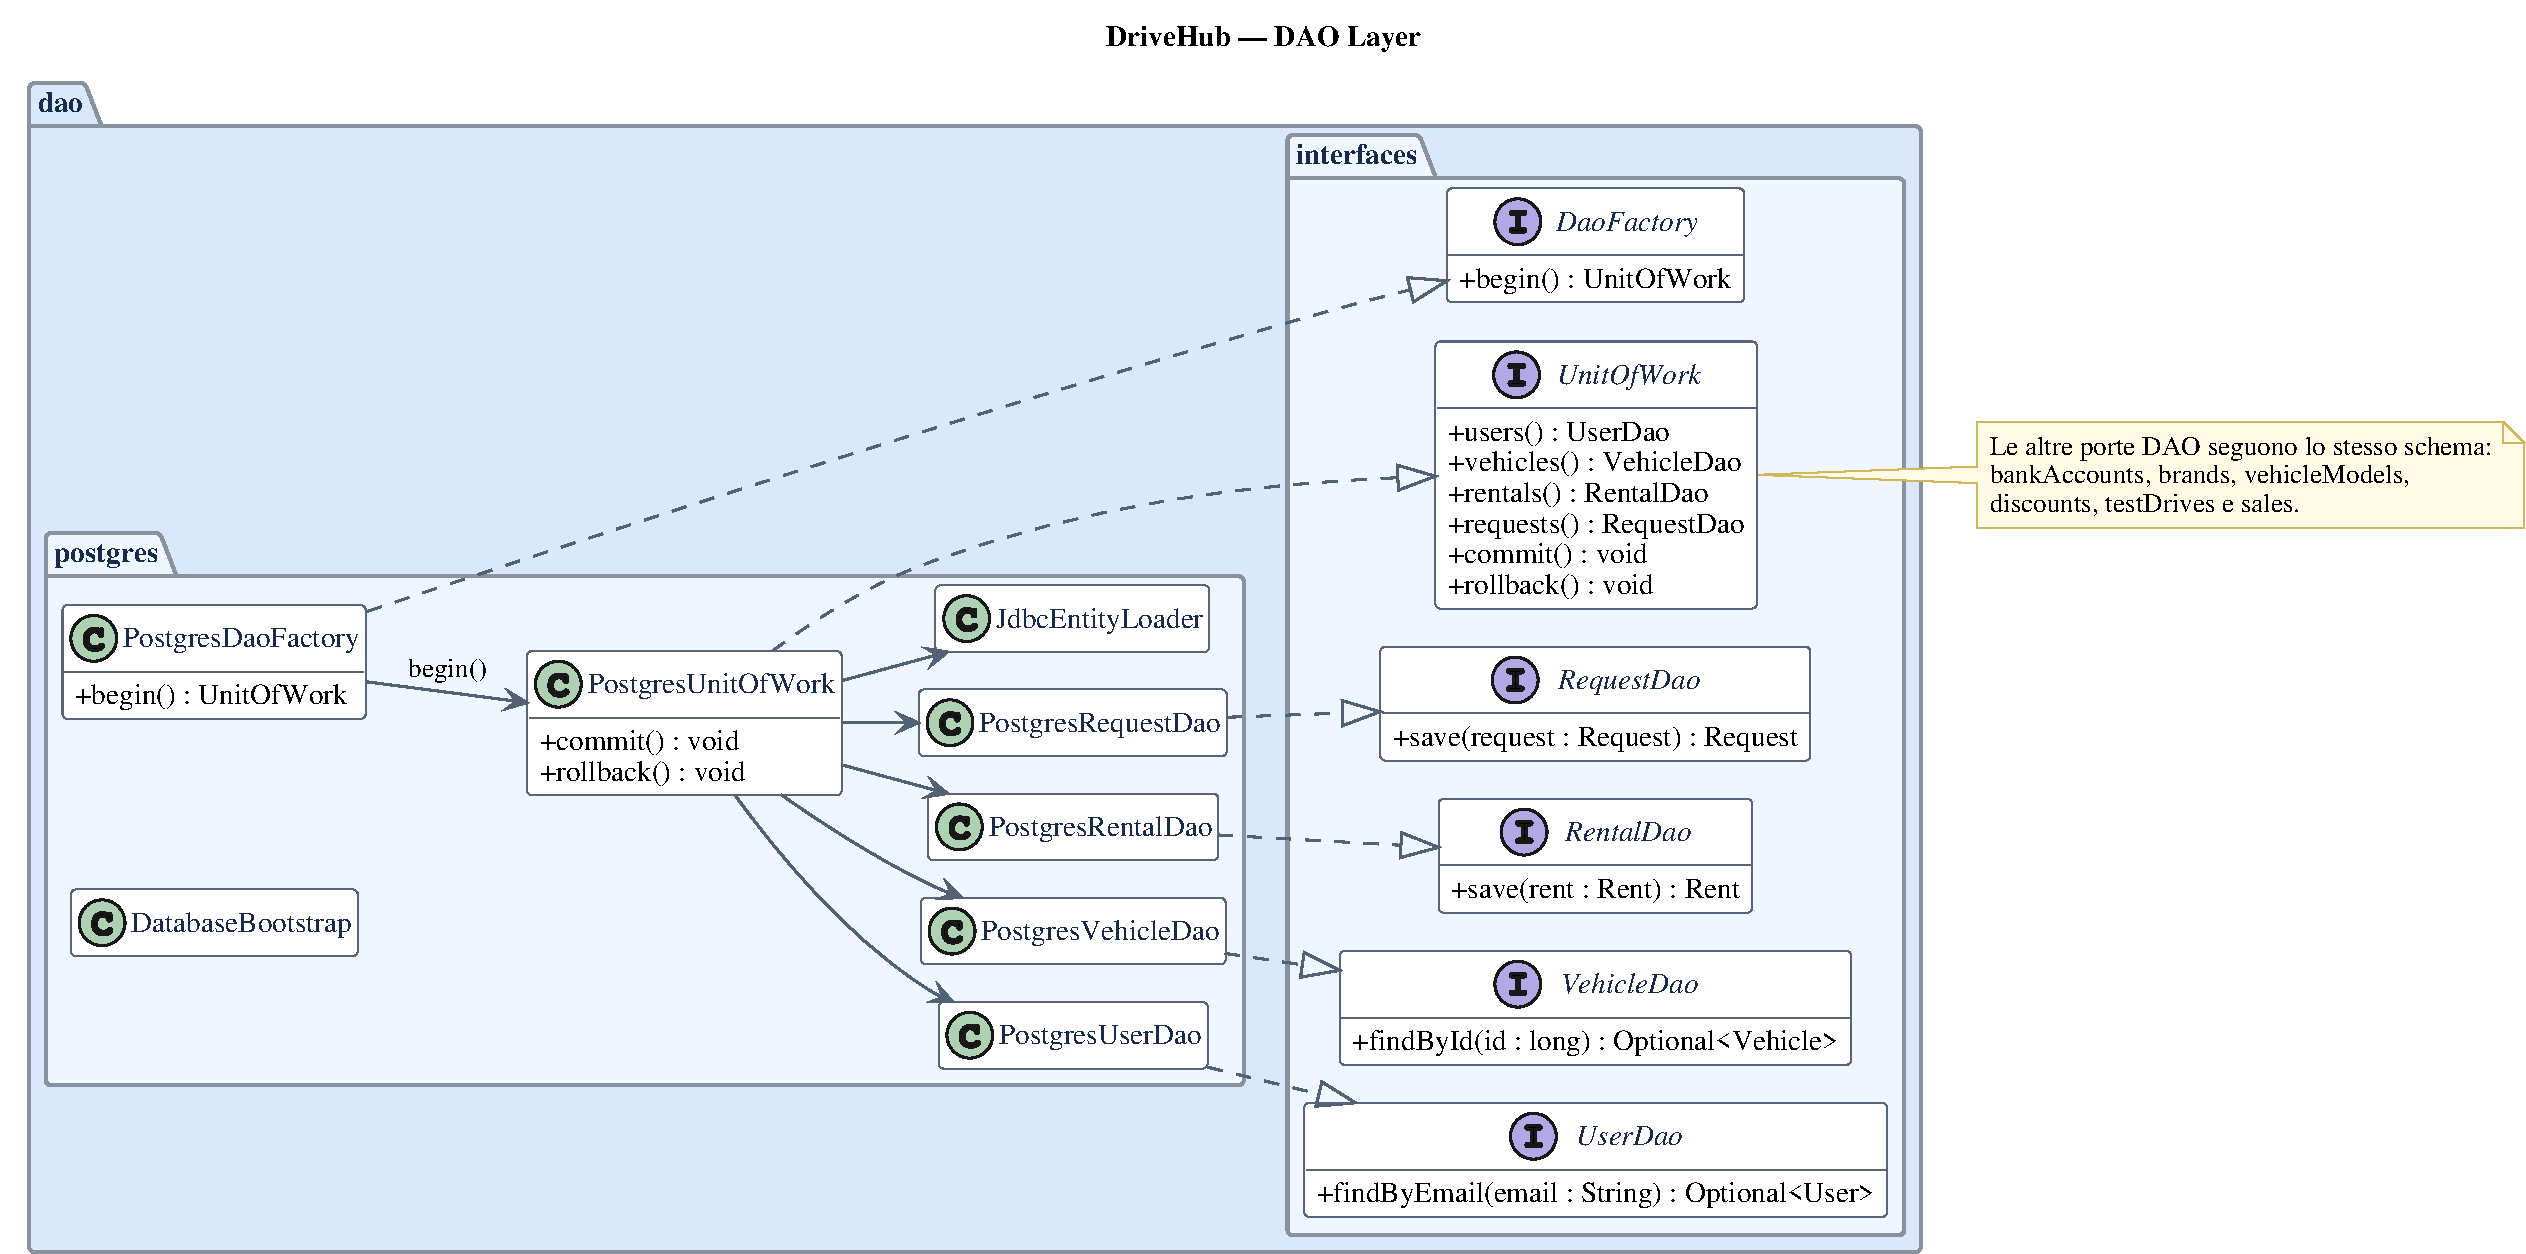
\includegraphics[width=\textwidth,height=.72\textheight,keepaspectratio]{class-dao-drivehub.pdf}
  \caption{DAO: porte, factory, unità di lavoro e implementazioni PostgreSQL rappresentative.}\label{fig:classi-dao}
\end{figure}

\clearpage
\subsection{Presentation Layer}

La presentazione raccoglie i controller JavaFX, il contesto applicativo, il gateway e la navigazione. I controller dei tre ruoli, del login e della registrazione estendono \code{AbstractController}, che riceve \code{ApplicationContext} e permette l'accesso a \code{UiGateway} e alla sessione. \code{ServiceUiGateway} implementa il gateway, invoca i servizi e restituisce i record di \code{UiModels}. \code{NavigationManager} carica le schermate individuate da \code{Route} e passa il contesto ai controller; \code{WelcomeController} è una classe separata, senza ereditarietà da \code{AbstractController}. Il controllo dei ruoli in \code{Route} riguarda la navigazione e non costituisce, da solo, un'autorizzazione di tutte le operazioni applicative.

\begin{figure}[H]
  \centering
  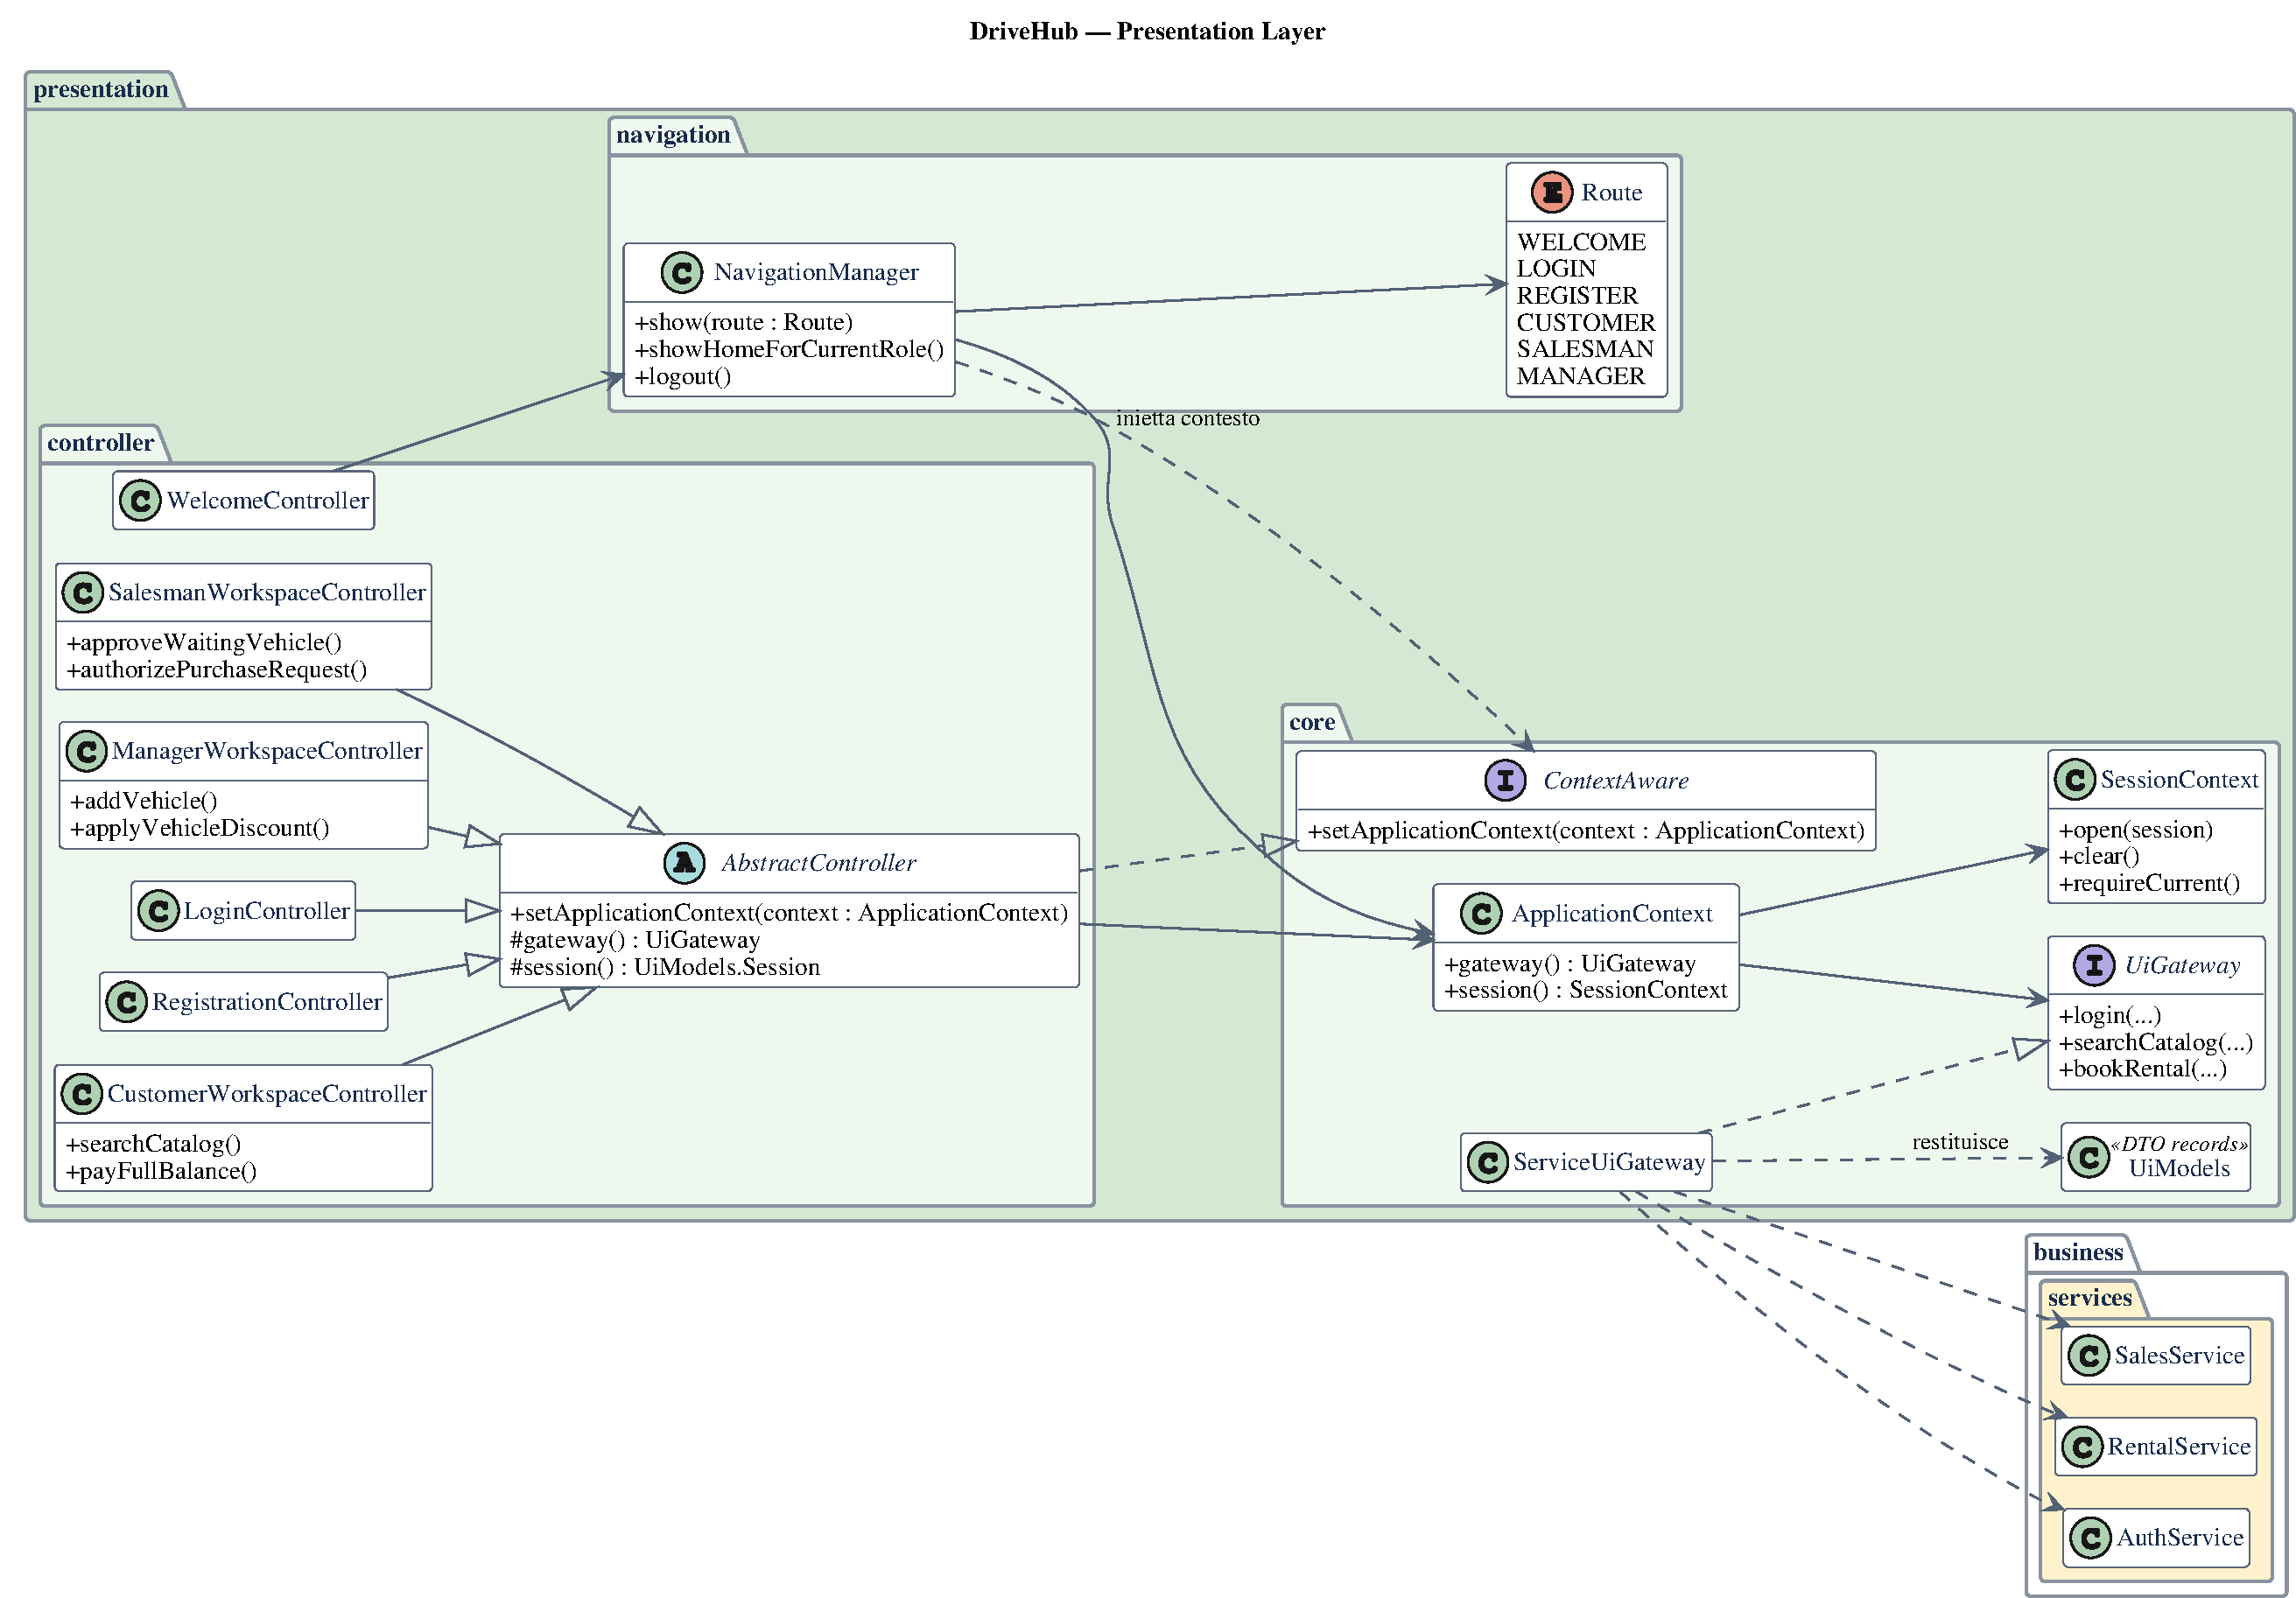
\includegraphics[width=\textwidth,height=.72\textheight,keepaspectratio]{class-presentation-drivehub.pdf}
  \caption{Presentation Layer: controller, gateway, sessione e navigazione.}\label{fig:classi-presentation}
\end{figure}
